\subsection{Negative Weights}
The negative weight problem is a well known problem in the world of ML-analysis for HEP, 
and is a consequence of higher perturbative accuracy. For the purpose of visualizing 
distributions, negative weights are not a problem. But, when using the weights in the 
training of the classifier, the XGBoost framework will not work. 
\\
Before deciding how to mediate the issue, I decided to plot the distribution for 
a small subset of features for all the events with negative weights.
\\
In figure \ref{fig:lep1_Pt_Neg} I plotted the absolute value $P_t$ distribution of events with
negative weights and compare it to all the events in figure \ref{fig:lep1_Pt_nNeg}. Similarly
I have plotted the same values for the second lepton in figures \ref{fig:lep1_Pt_nNeg} and \ref{fig:lep2_Pt_nNeg}
respectively. From the two comparisons we see that the distribution of negative
weights is relatively equal to that of all the events. The same comparisons have
been made in figures \ref{fig:lep1_Phi_Neg}, \ref{fig:lep1_Phi_nNeg}, \ref{fig:lep2_Phi_nNeg}  
and \ref{fig:lep2_Phi_nNeg} respectively but for $\phi$. The same obsorvations
are made for both $P_t$ and $\phi$. This means we can be justified in treating the 
negative weight distribution uniformally across the feature space.
\begin{figure}
    \makebox[0.9\linewidth][c]{%
    \centering
    \begin{subfigure}{.425\textwidth}
        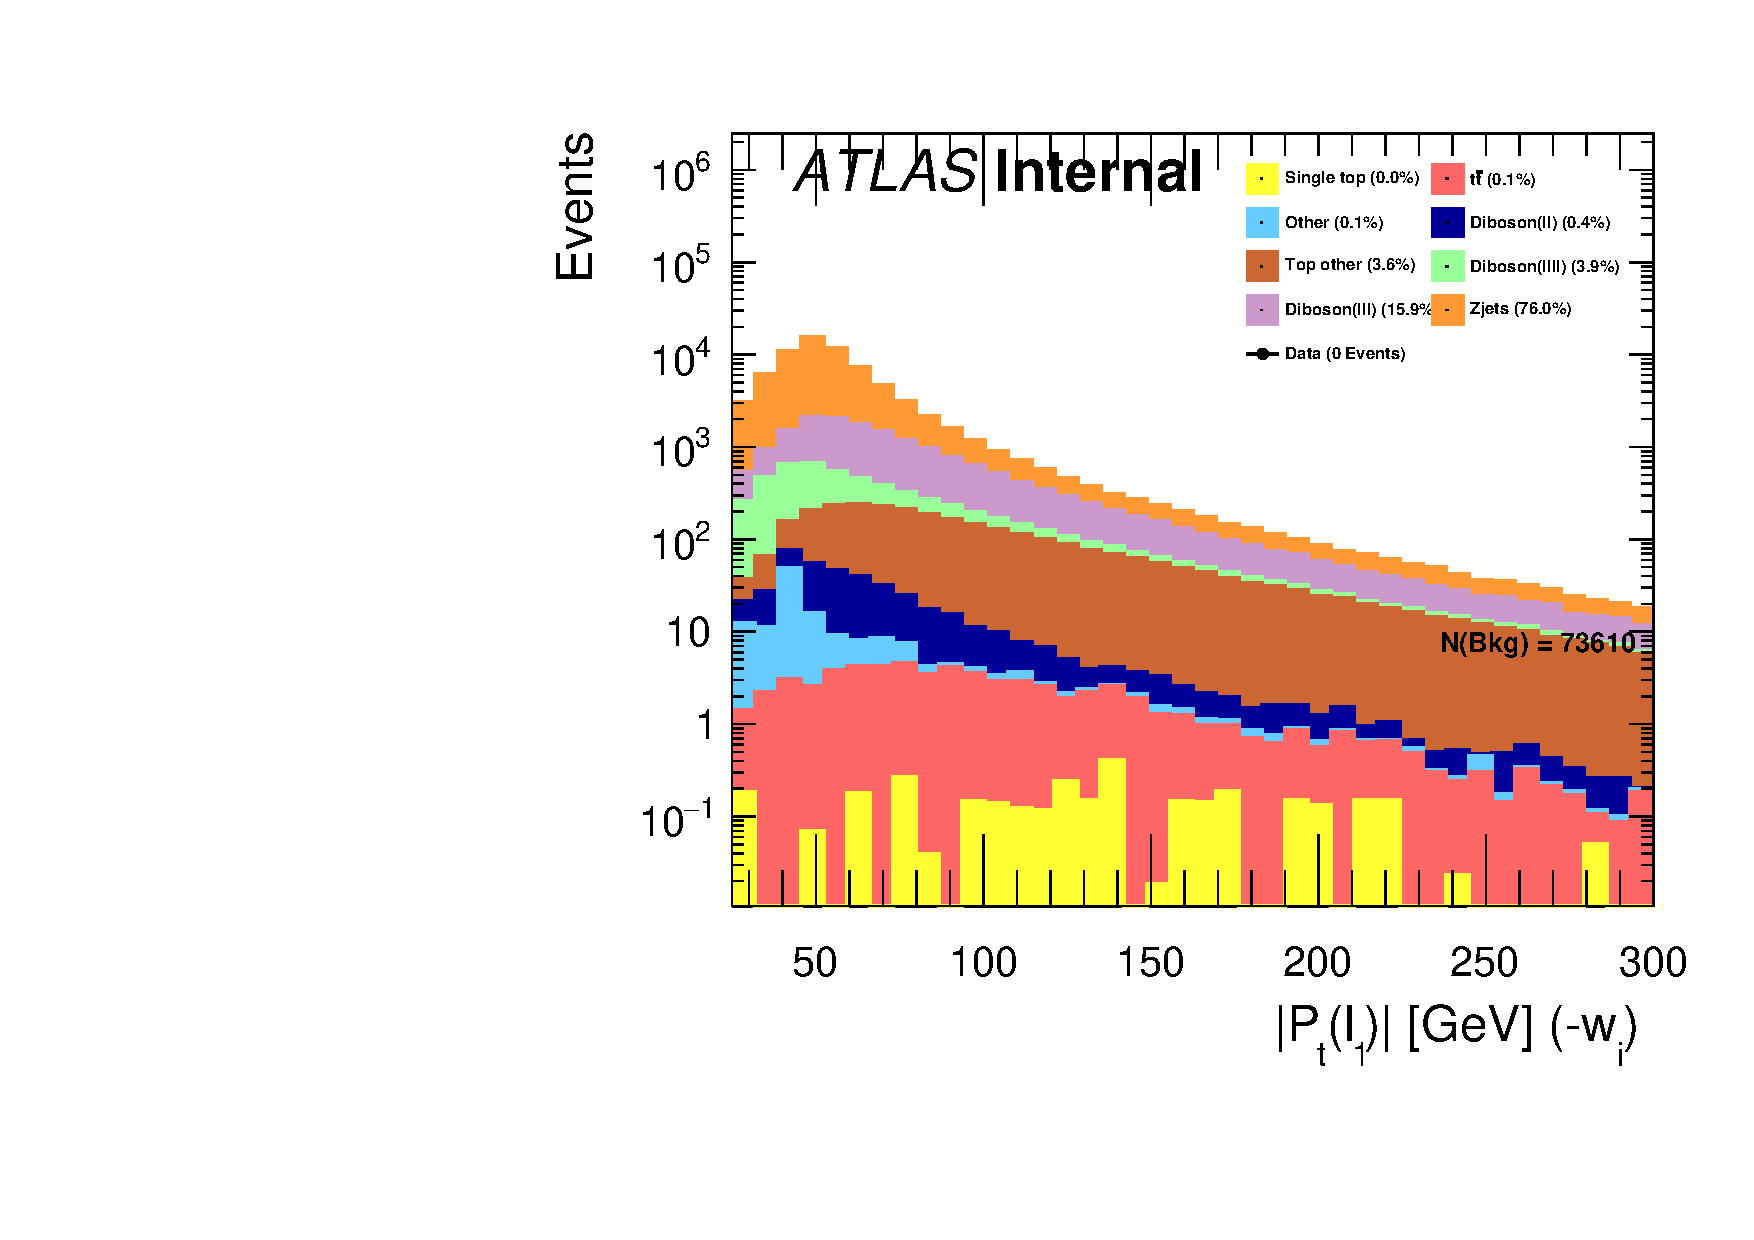
\includegraphics[width=\textwidth]{Figures/FeaturesHistograms/lep1_Pt_Neg.pdf}
        \caption{}
        \label{fig:lep1_Pt_Neg}
    \end{subfigure}
    \hfill
    \begin{subfigure}{.425\textwidth}
        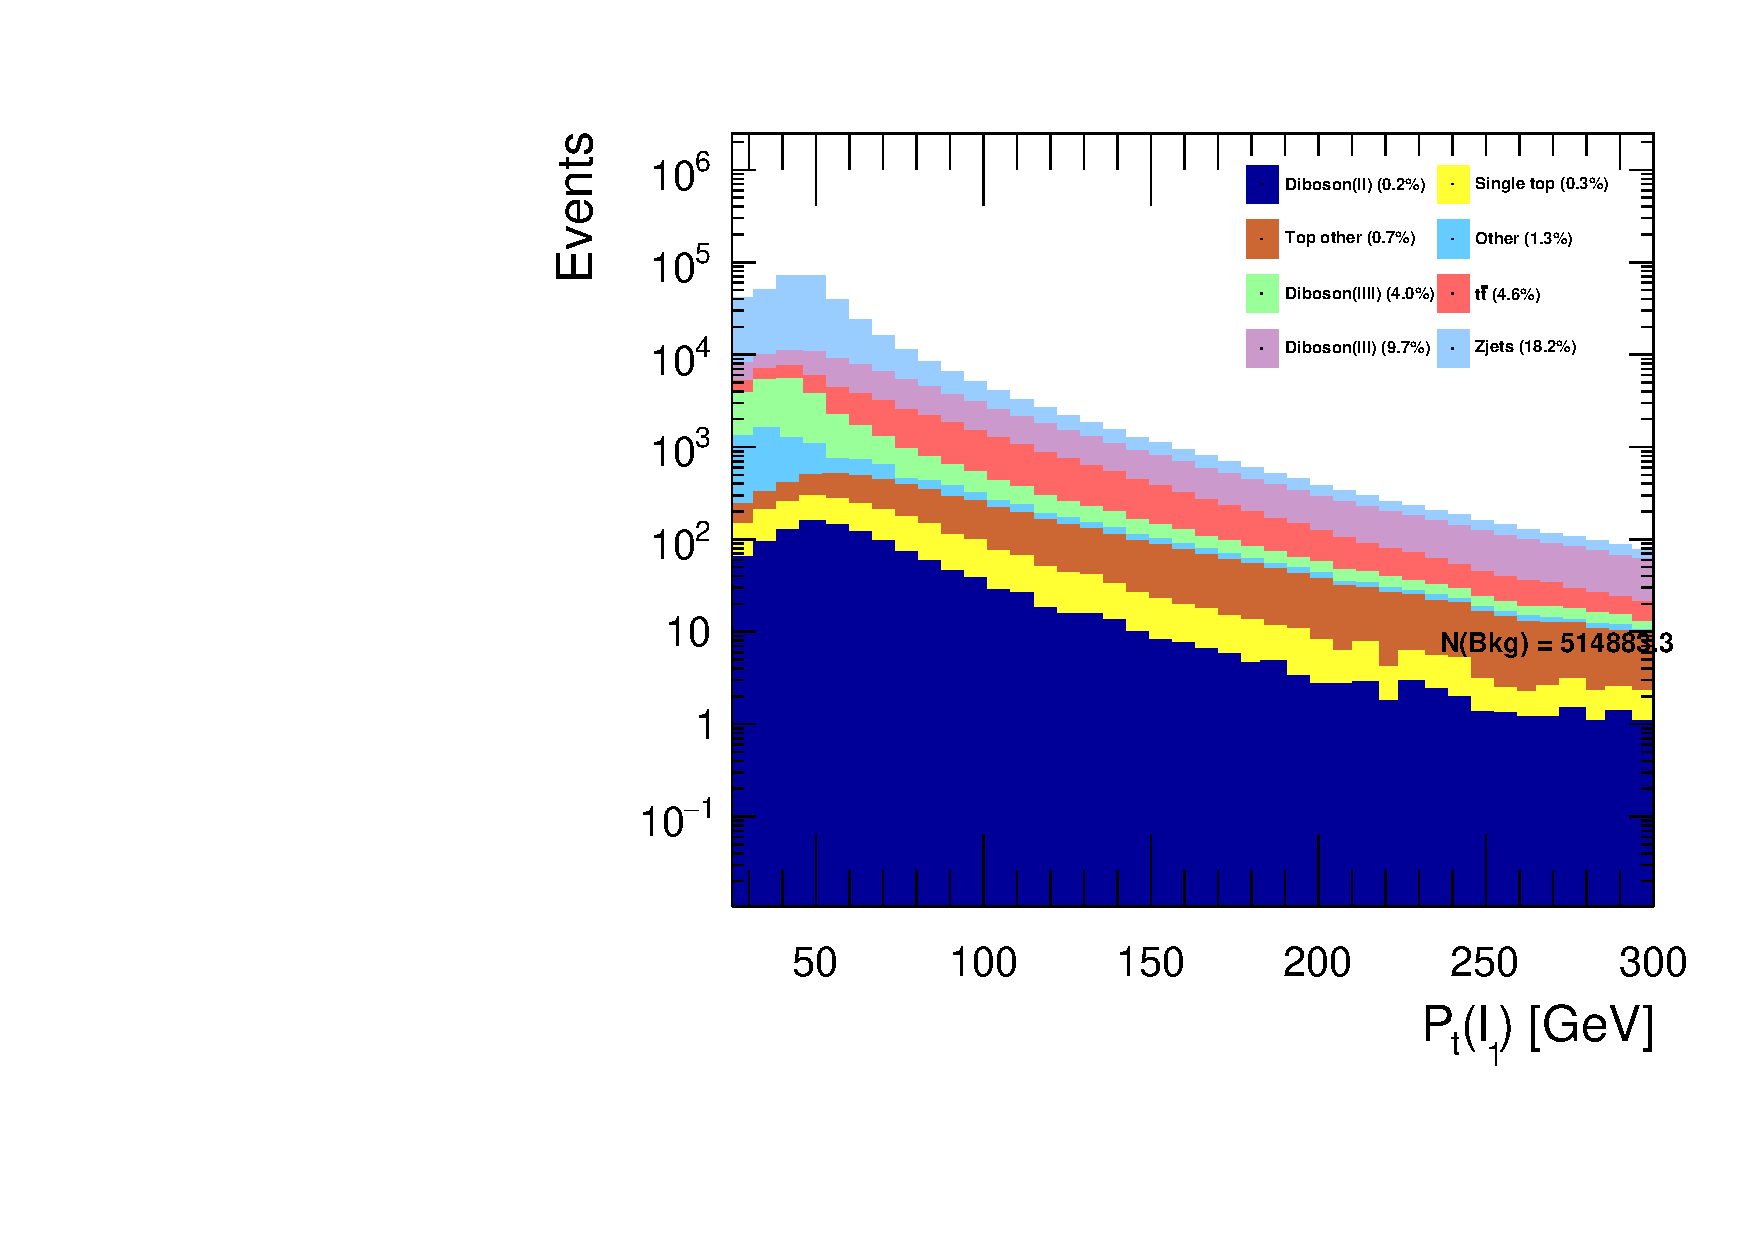
\includegraphics[width=\textwidth]{Figures/FeaturesHistograms/lep1_Pt_nNeg.pdf}
        \caption{}
        \label{fig:lep1_Pt_nNeg}
    \end{subfigure}
    }
    \makebox[0.9\linewidth][c]{%
    \begin{subfigure}{.425\textwidth}
        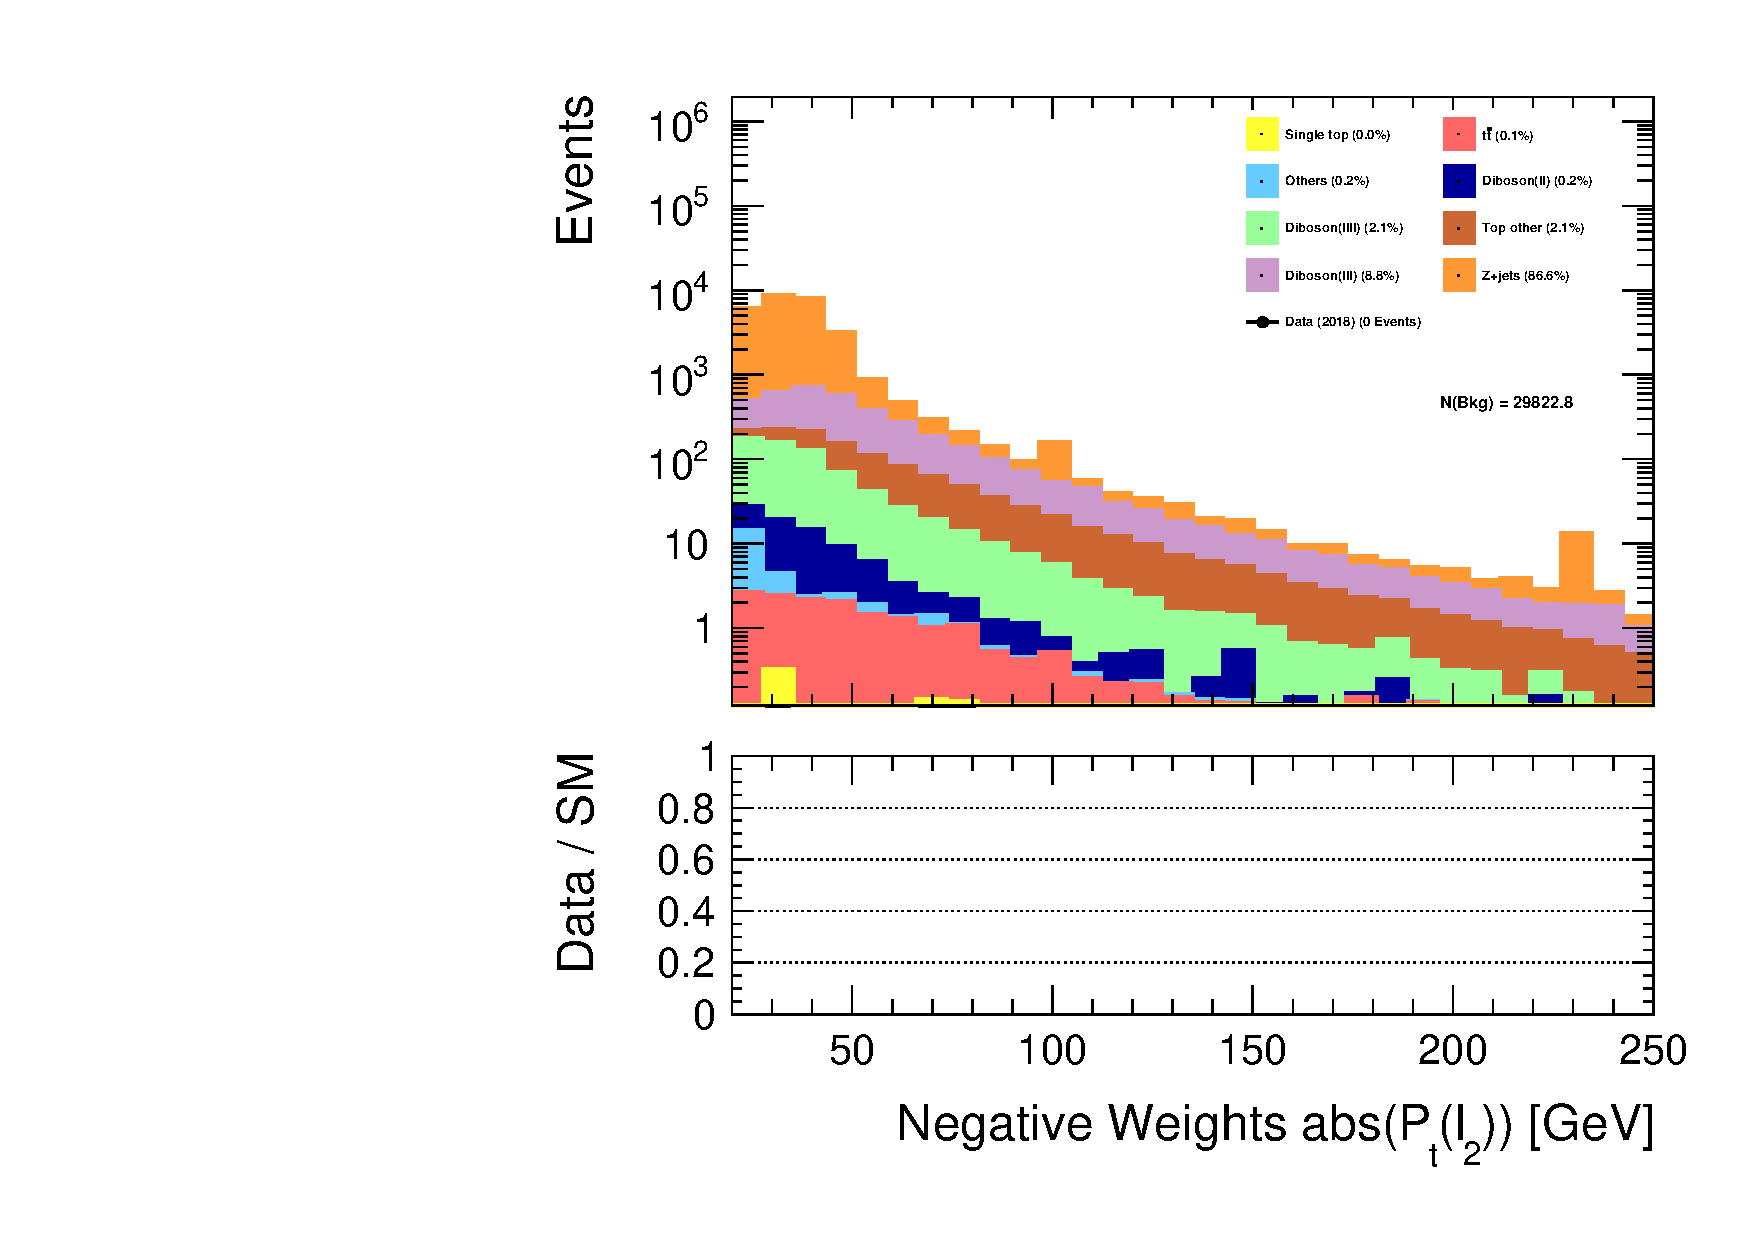
\includegraphics[width=\textwidth]{Figures/FeaturesHistograms/lep2_Pt_Neg.pdf}
        \caption{}
        \label{fig:lep2_Pt_Neg}
    \end{subfigure}
    \hfill
    \begin{subfigure}{.425\textwidth}
        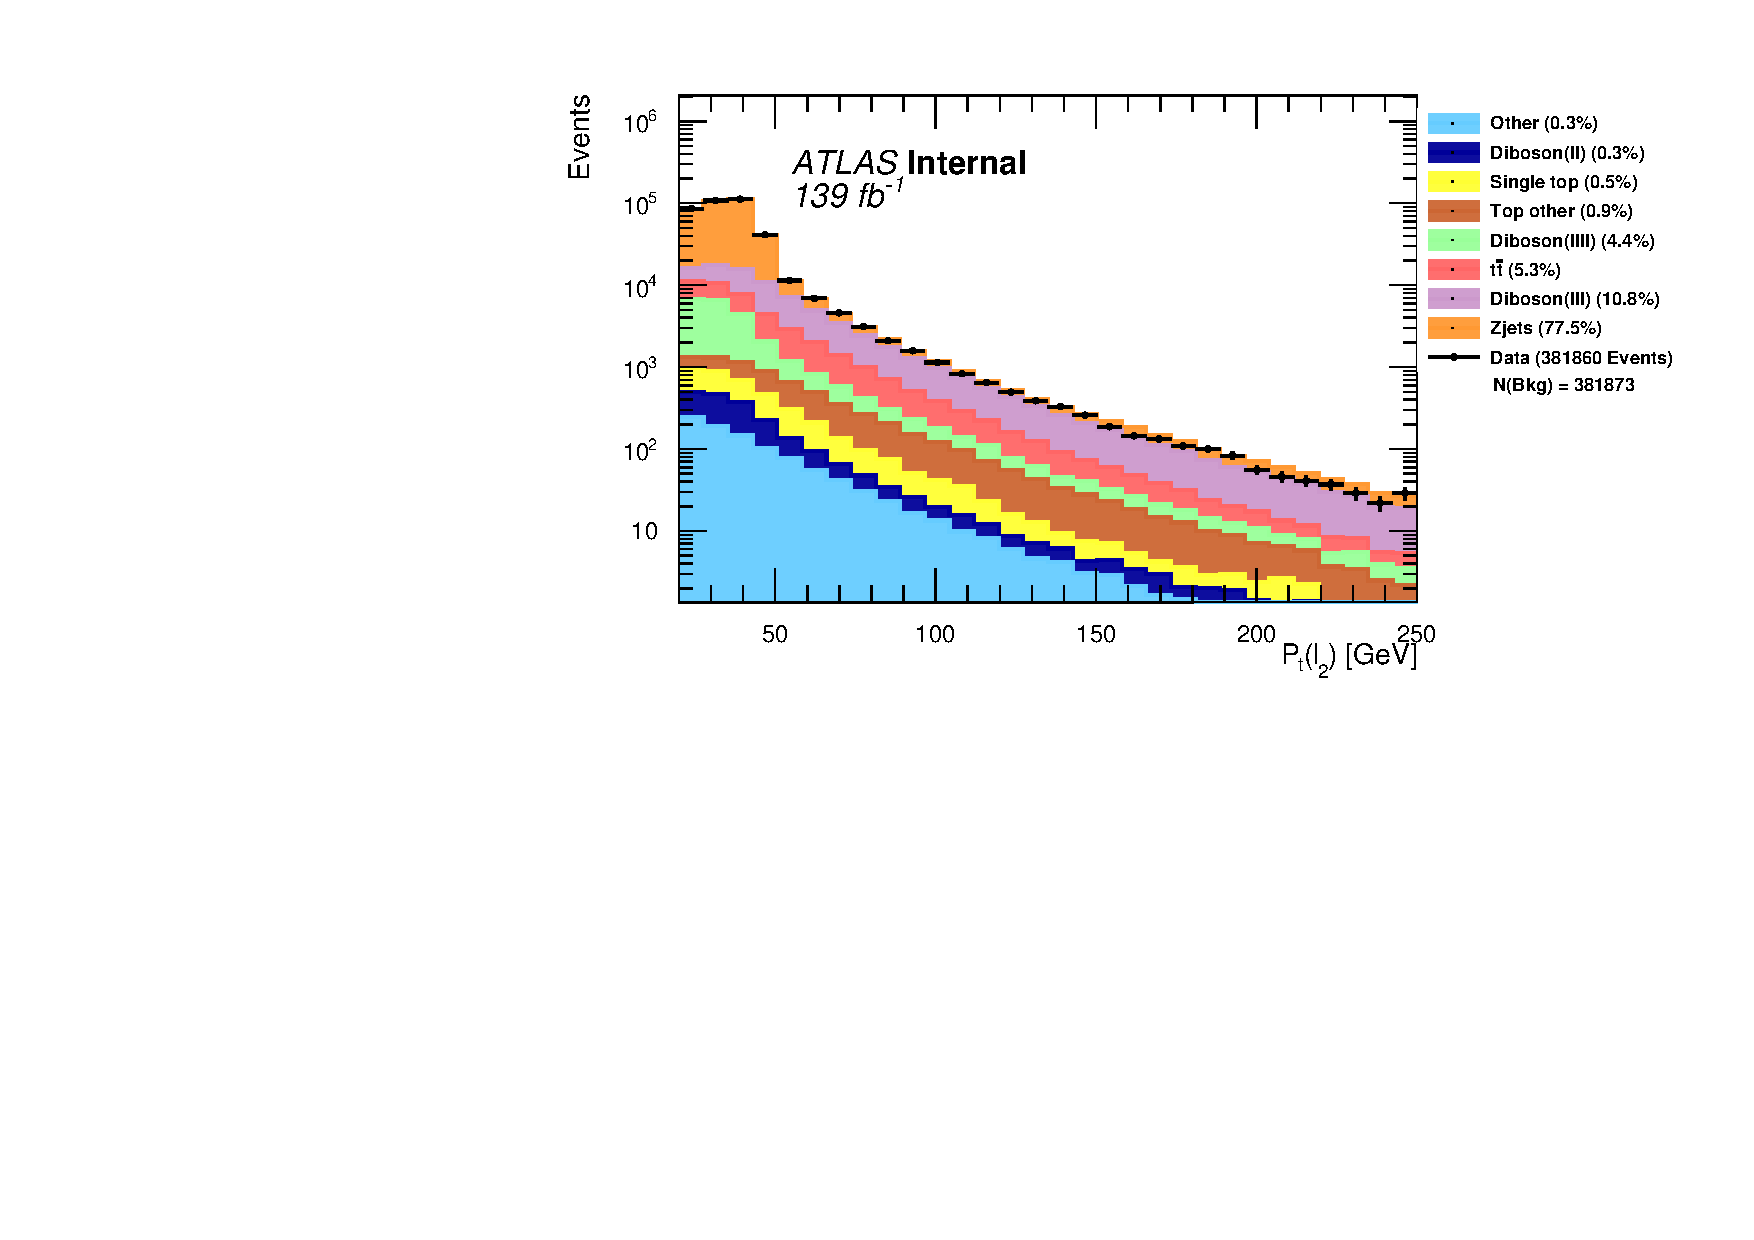
\includegraphics[width=\textwidth]{Figures/FeaturesHistograms/lep2_Pt_nNeg.pdf}
        \caption{ }
        \label{fig:lep2_Pt_nNeg}
    \end{subfigure}
    }
    \caption{The absolute value of the $P_t$ for events with stricly negative weights 
    ($l_1$ \ref{fig:lep1_Pt_Neg}, $l_2$ \ref{fig:lep2_Pt_Neg}) and all events
    ($l_1$ \ref{fig:lep1_Pt_nNeg}, $l_2$ \ref{fig:lep2_Pt_nNeg}). }
\end{figure}

\begin{figure}
    \makebox[0.9\linewidth][c]{%
    \centering
    \begin{subfigure}{.425\textwidth}
        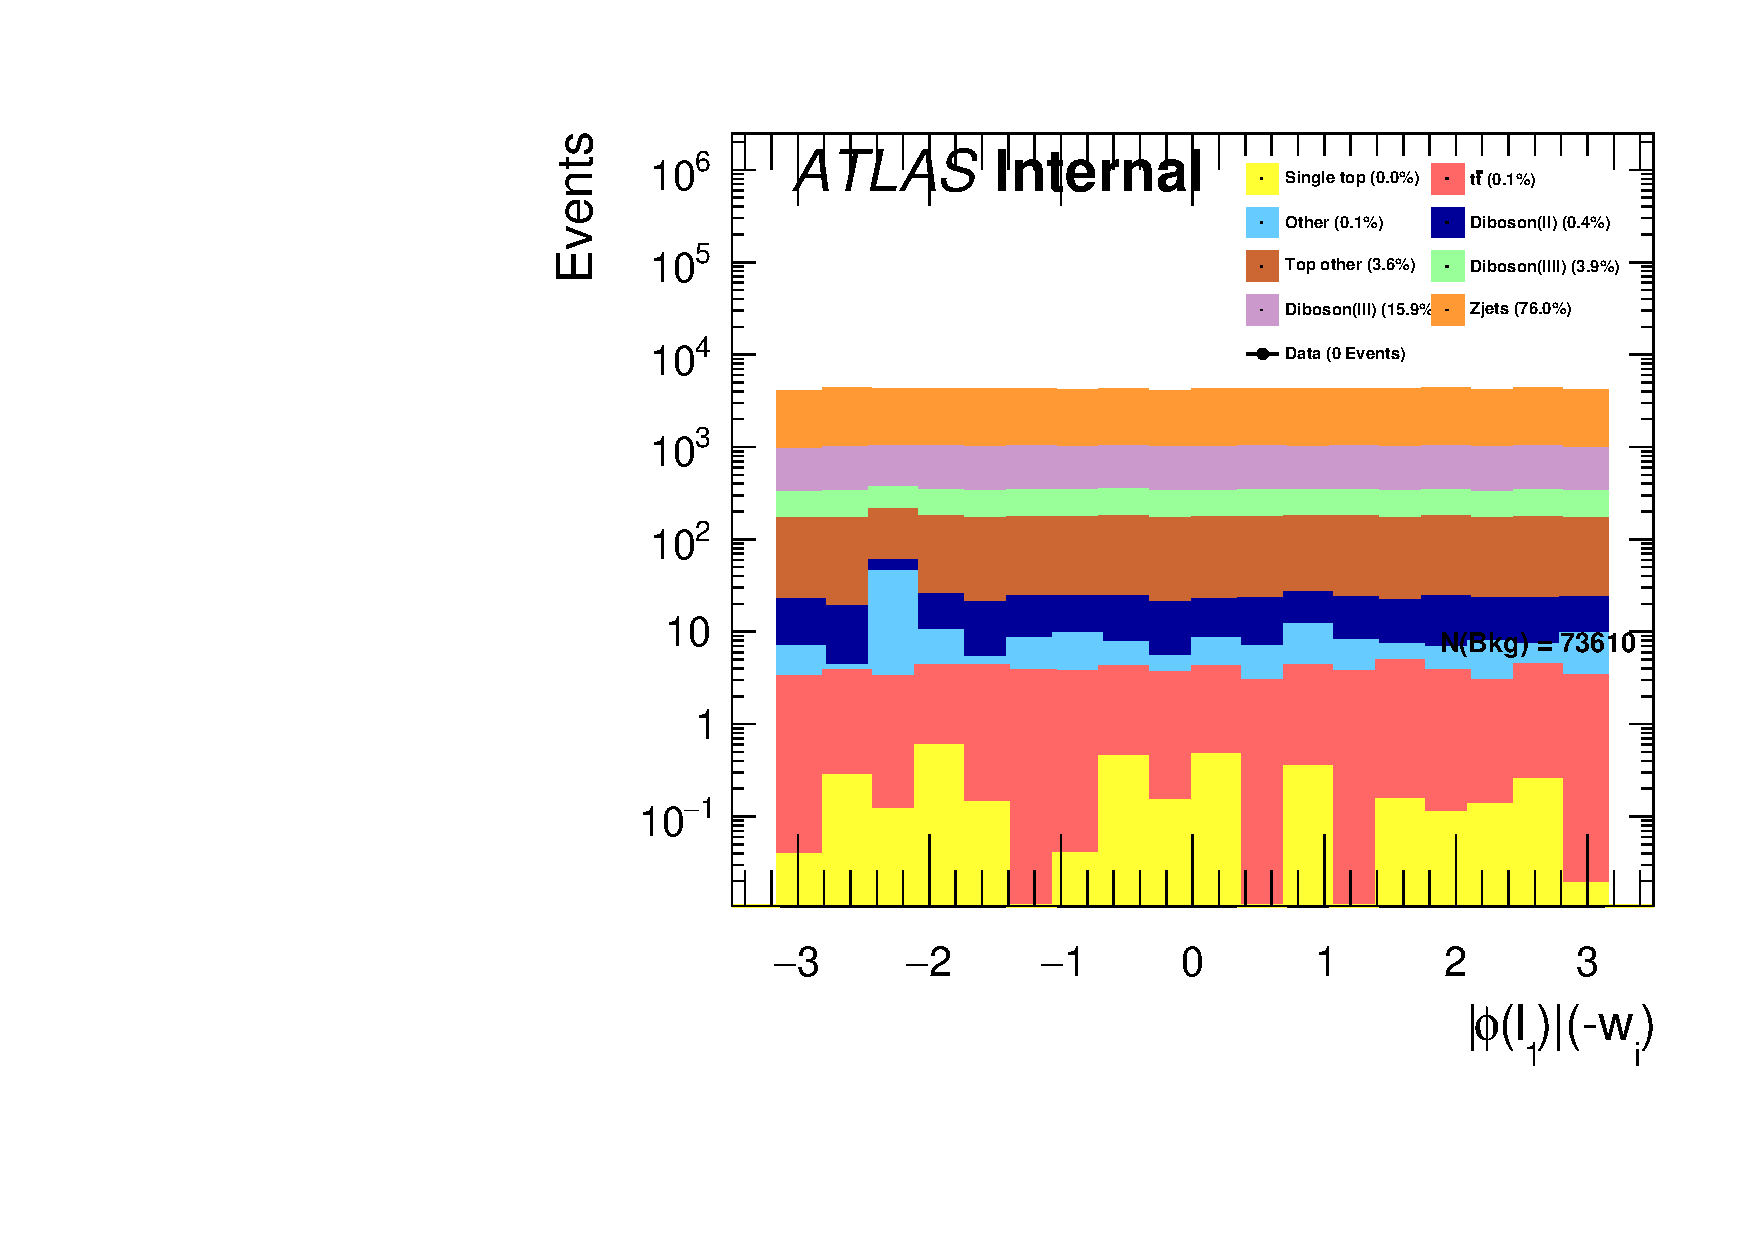
\includegraphics[width=\textwidth]{Figures/FeaturesHistograms/lep1_Phi_Neg.pdf}
        \caption{}
        \label{fig:lep1_Phi_Neg}
    \end{subfigure}
    \hfill
    \begin{subfigure}{.425\textwidth}
        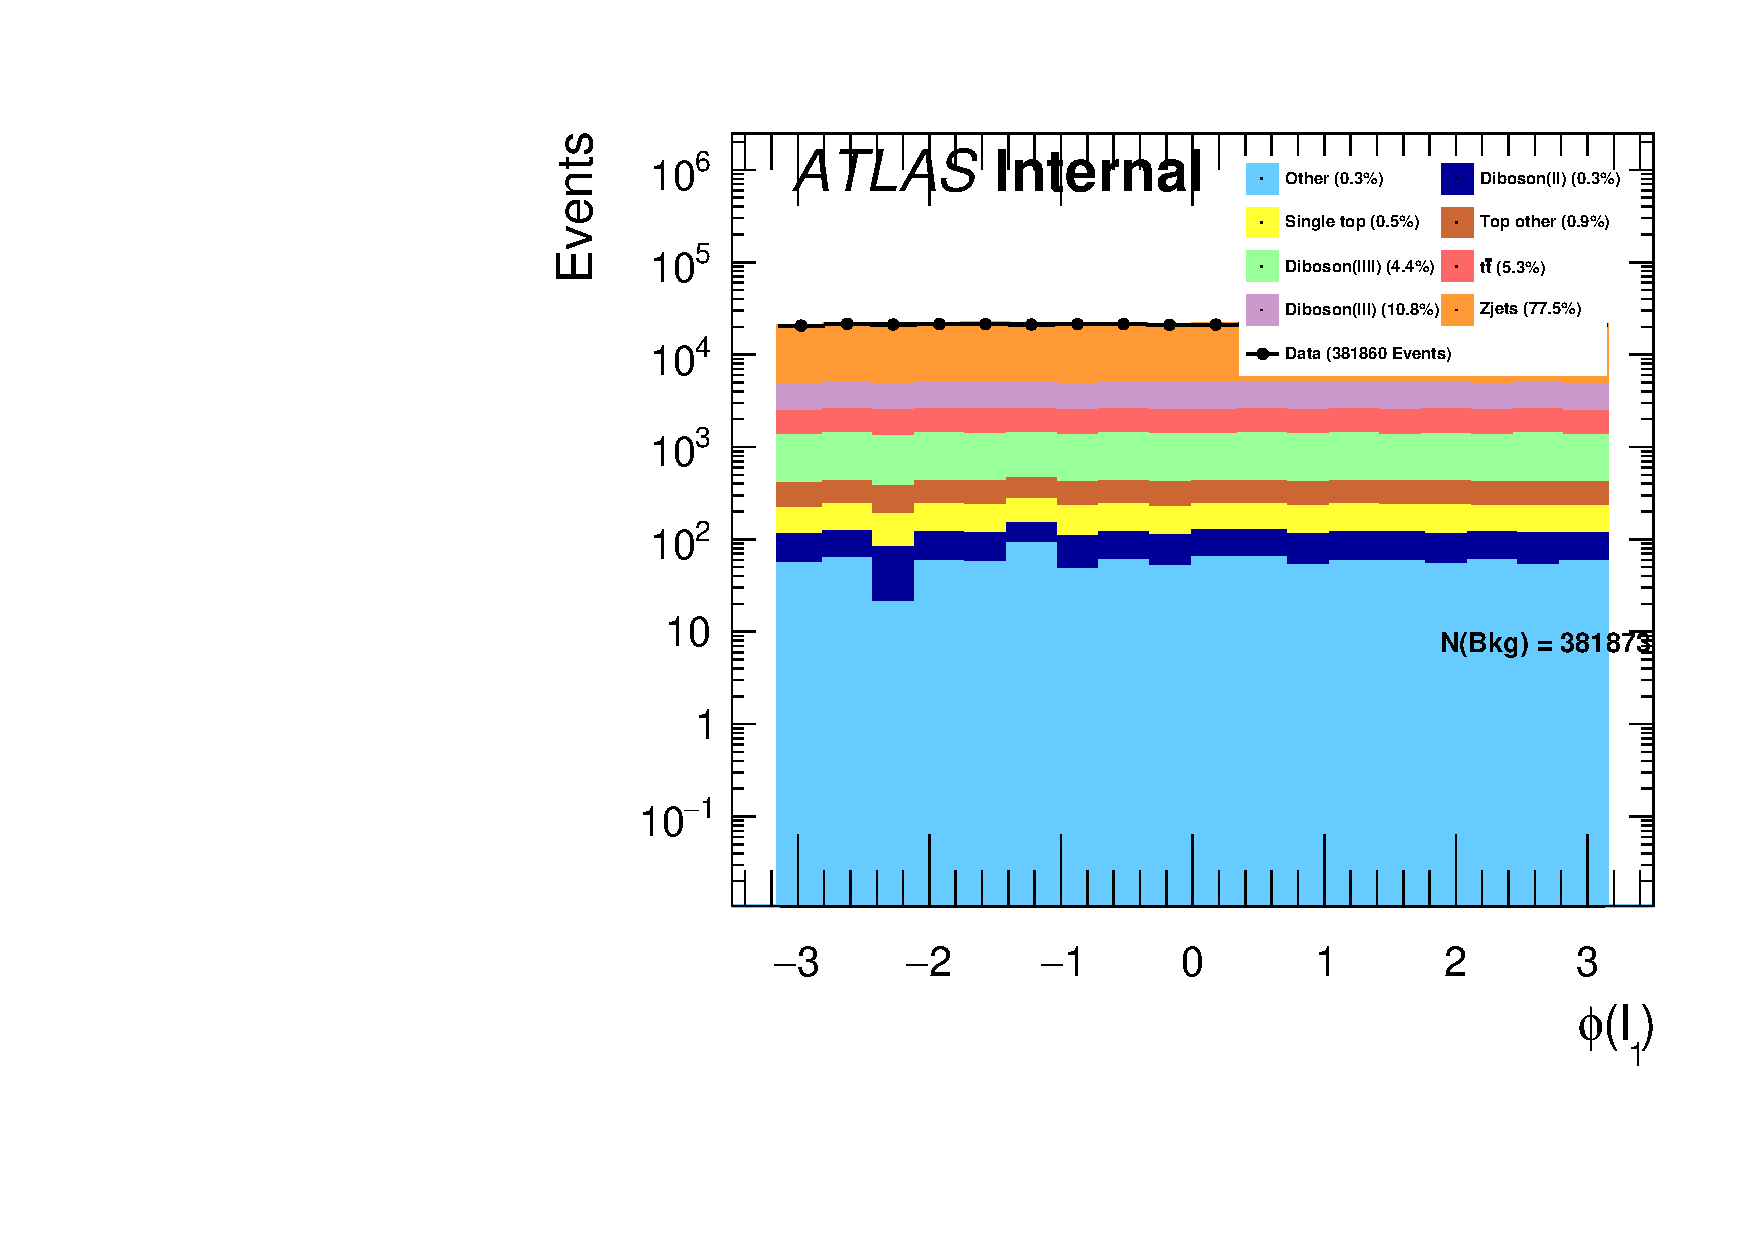
\includegraphics[width=\textwidth]{Figures/FeaturesHistograms/lep1_Phi_nNeg.pdf}
        \caption{}
        \label{fig:lep1_Phi_nNeg}
    \end{subfigure}
    }
    \makebox[0.9\linewidth][c]{%
    \begin{subfigure}{.425\textwidth}
        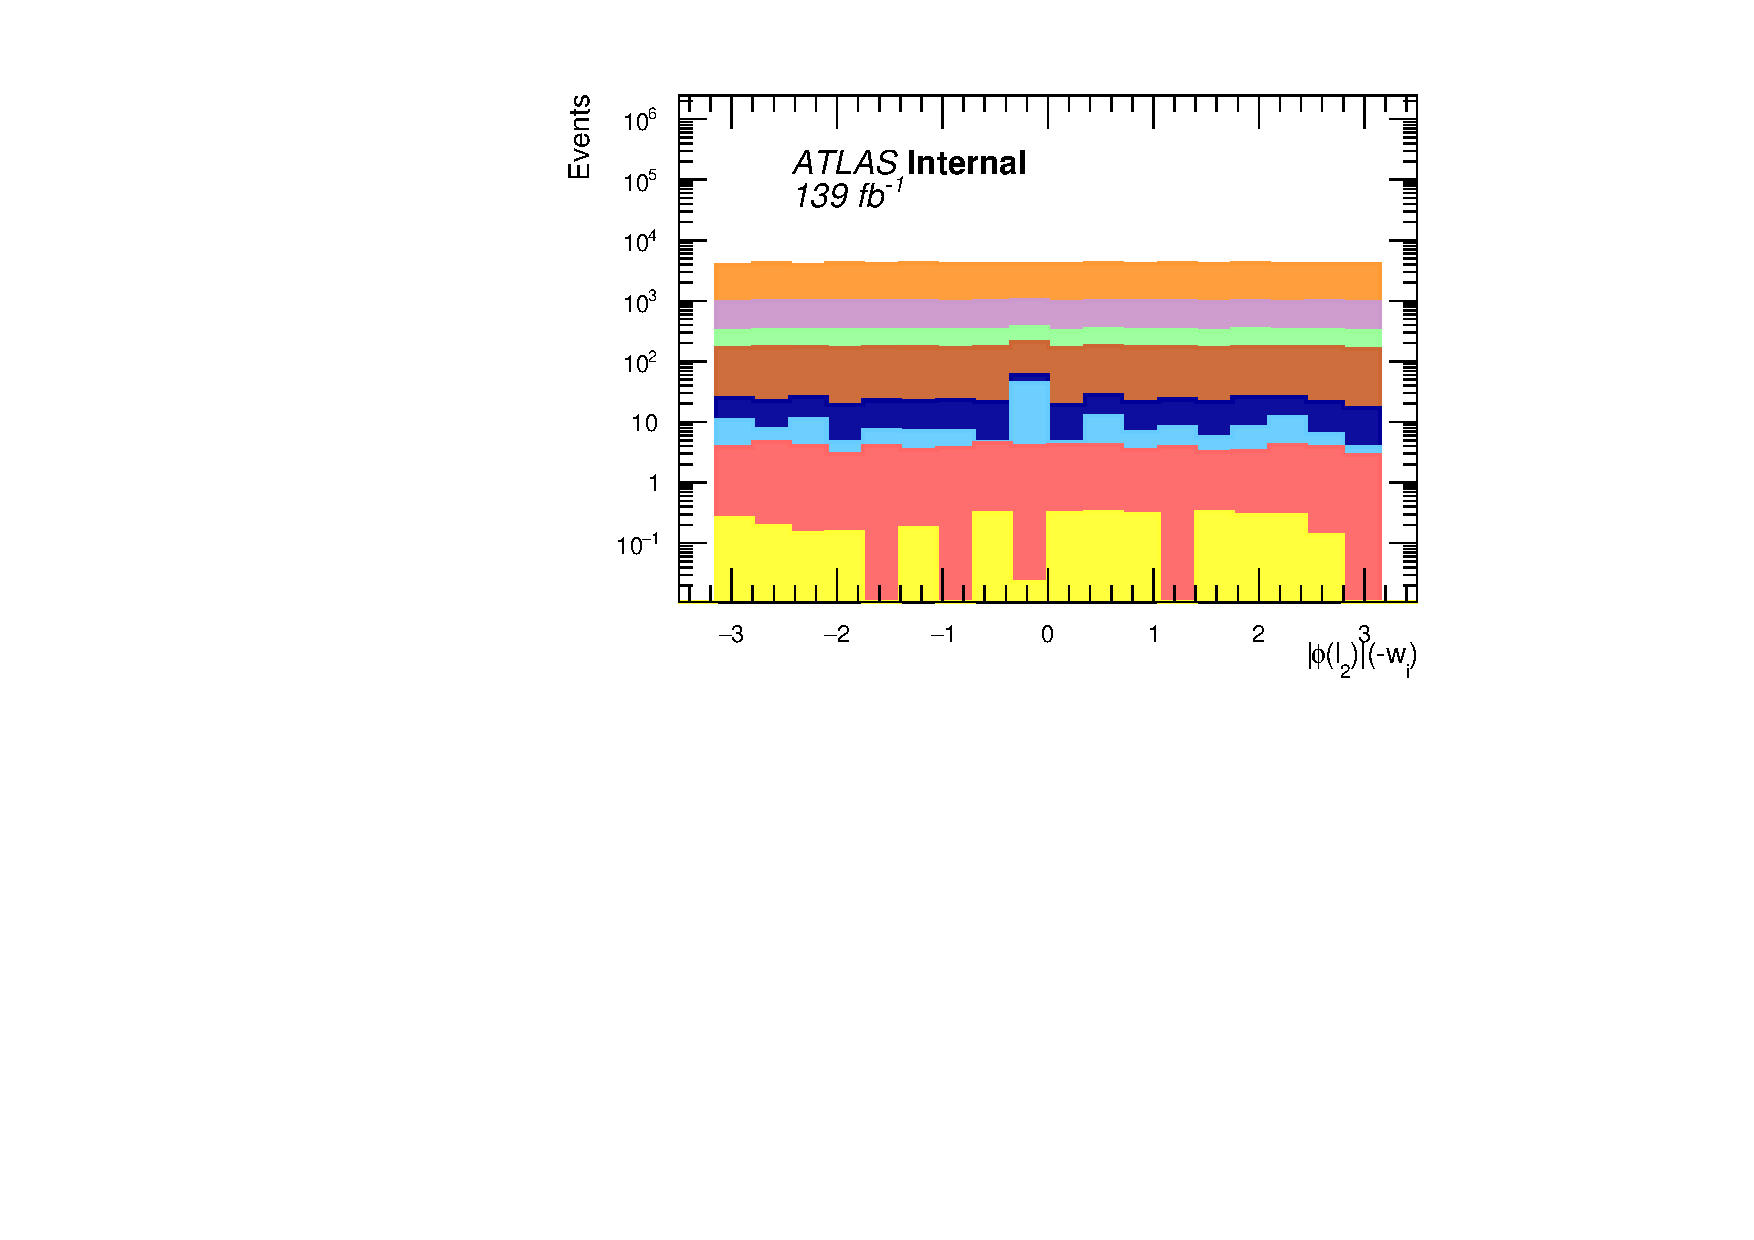
\includegraphics[width=\textwidth]{Figures/FeaturesHistograms/lep2_Phi_Neg.pdf}
        \caption{}
        \label{fig:lep2_Phi_Neg}
    \end{subfigure}
    \hfill
    \begin{subfigure}{.425\textwidth}
        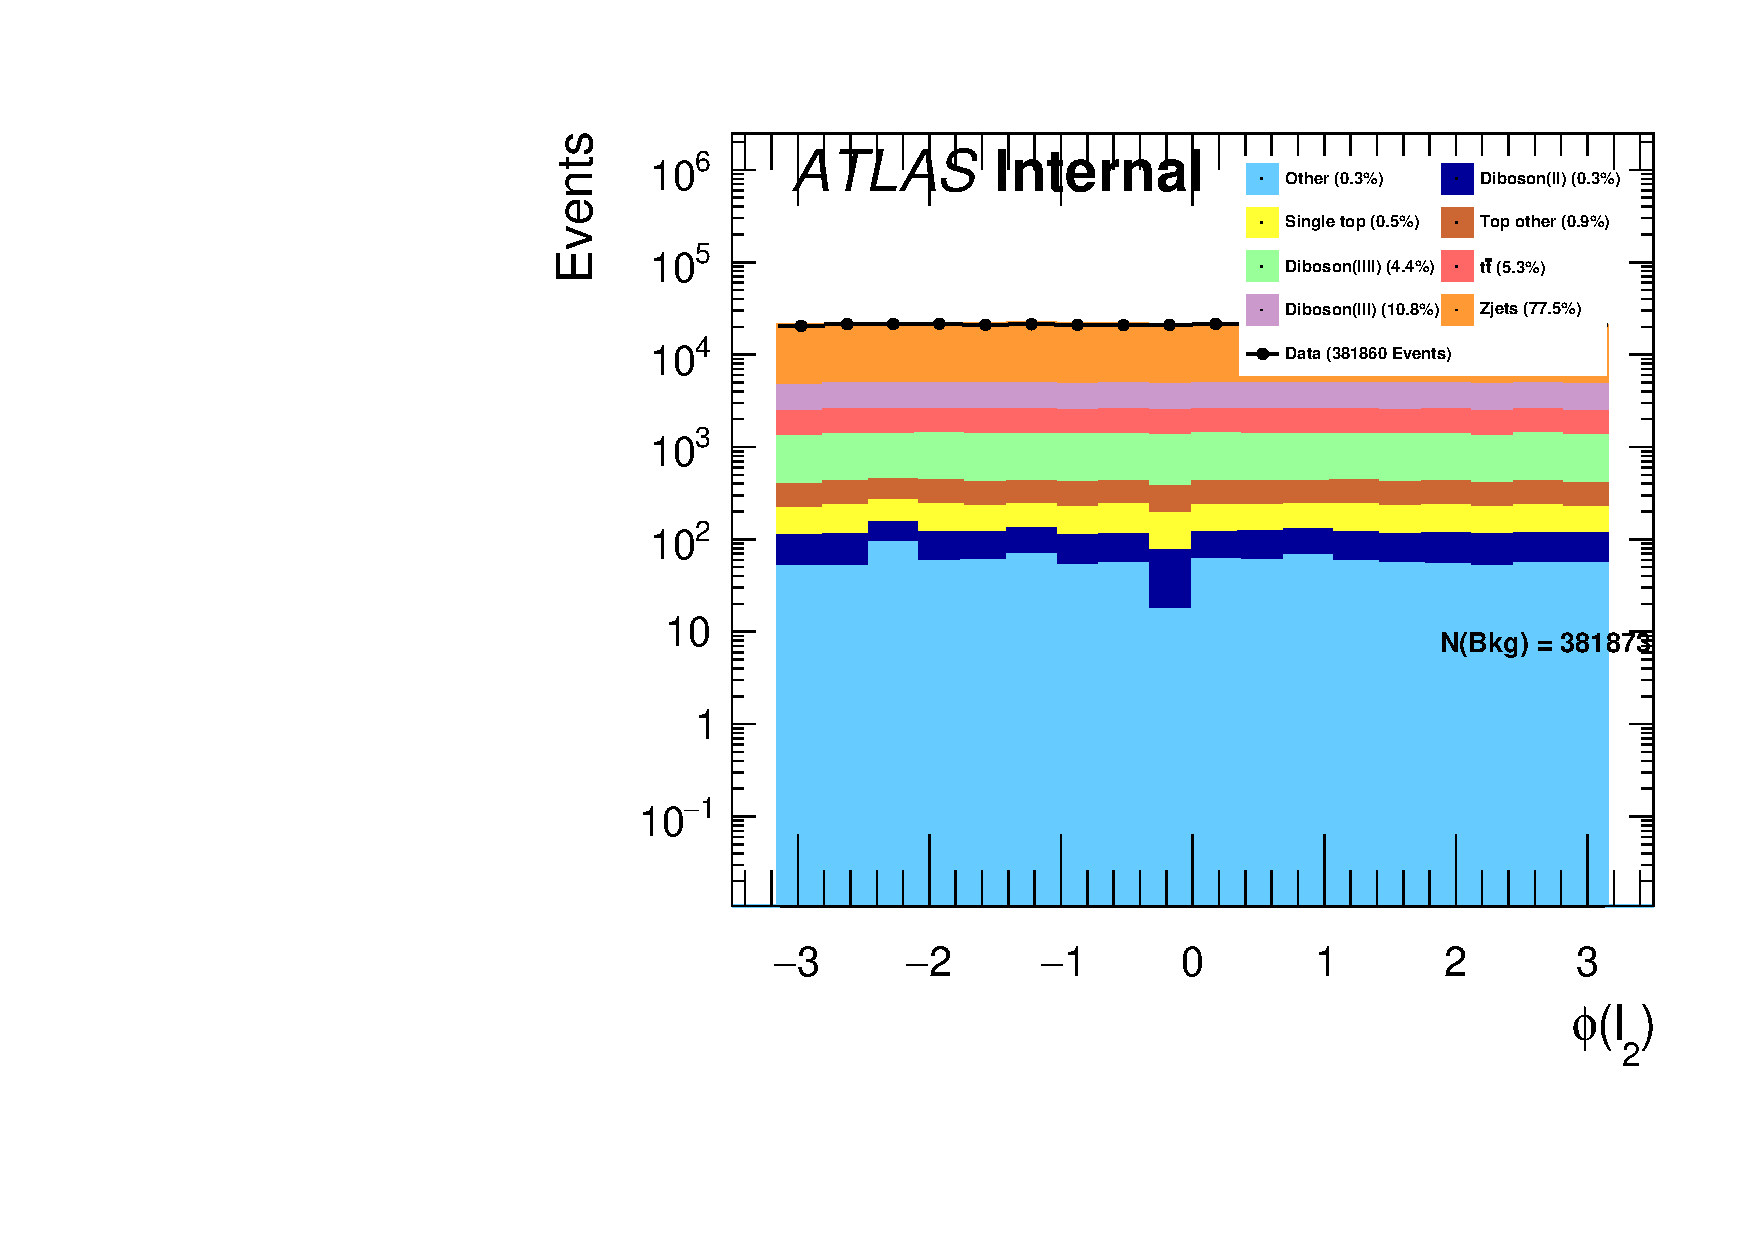
\includegraphics[width=\textwidth]{Figures/FeaturesHistograms/lep2_Phi_nNeg.pdf}
        \caption{}
        \label{fig:lep2_Phi_nNeg}
    \end{subfigure}
    }
    \caption{The absolute value of the $\phi$ for events with strictly negative weights 
    ($l_1$ \ref{fig:lep1_Phi_Neg}, $l_2$ \ref{fig:lep2_Phi_Neg}) and all events
    ($l_1$ \ref{fig:lep1_Phi_nNeg}, $l_2$ \ref{fig:lep2_Phi_nNeg}). }

\end{figure}
How one chooses to deal with this problem can heavily effect results and many solutions 
are suggested as a consequence. Given the time main focus of this rapport, the 
simplest solution was chosen. Namely, I chose to normalize all the weights as a 
whole, conserving the total sum of the weights and at the same time changing all 
negative signs. The simple procedure is shown bellow in equation \ref{eq:negw},
\begin{align}\label{eq:negw}
    w_i & = P \mid w_i \mid\,  \\
    P  & =  \sum_{j=0}^{N-1}\frac{ w_j}{\mid w_j \mid},
\end{align}
where $w_i$ is the weight of an event i, $i \in [0,N-1]$ and N equals the total number of events.
Although this is a very simplistic solution, our observations made for the distribution
of negative weights can be used to justify the approach.


